
\documentclass{article} % For LaTeX2e
\usepackage{format/nips13submit_e}
\nipsfinalcopy % Uncomment for camera-ready version
\usepackage{times}
\usepackage{hyperref}
\usepackage{url}
\usepackage{color}
\definecolor{mydarkblue}{rgb}{0,0.08,0.45}
\hypersetup{ %
    pdftitle={},
    pdfauthor={},
    pdfsubject={},
    pdfkeywords={},
    pdfborder=0 0 0,
    pdfpagemode=UseNone,
    colorlinks=true,
    linkcolor=mydarkblue,
    citecolor=mydarkblue,
    filecolor=mydarkblue,
    urlcolor=mydarkblue,
    pdfview=FitH}
    
\usepackage{graphicx, amsmath, amsfonts, bm, lipsum, capt-of}

\usepackage{natbib, xcolor, wrapfig, booktabs, multirow, caption}

\usepackage{float}

\usepackage{titlesec}
\newcommand{\sectionbreak}{\clearpage}
\newcommand{\subsectionbreak}{\clearpage}
\pagenumbering{gobble}
\def\ie{i.e.\ }
\def\eg{e.g.\ }

\title{An automatic report for the dataset : 02-solar}

\author{
James Robert Lloyd\\
University of Cambridge\\
Department of Engineering\\
\texttt{jrl44@cam.ac.uk}
\And
David Duvenaud\\
University of Cambridge \\
Department of Engineering \\
\texttt{dkd23@cam.ac.uk} \\
\And
Roger Grosse\\
M.I.T.\\
Brain and Cognitive Sciences \\
\texttt{rgrosse@mit.edu}
\And
Joshua B. Tenenbaum\\
M.I.T.\\
Brain and Cognitive Sciences \\
\texttt{jbt@mit.edu}
\And
Zoubin Ghahramani\\
University of Cambridge \\
Department of Engineering \\
\texttt{zoubin@eng.cam.ac.uk}
}

\newcommand{\fix}{\marginpar{FIX}}
\newcommand{\new}{\marginpar{NEW}}

\setlength{\marginparwidth}{0.9in}
%%%%%%%%%%%%%%%%%%%%%%%%%%%%%%%%%%%%%%%%%%%%%%%%%%%%%%%%%%
%%%% EDITING HELPER FUNCTIONS  %%%%%%%%%%%%%%%%%%%%%%%%%%%
%%%%%%%%%%%%%%%%%%%%%%%%%%%%%%%%%%%%%%%%%%%%%%%%%%%%%%%%%%

%% NA: needs attention (rough writing whose correctness needs to be verified)
%% TBD: instructions for how to fix a gap ("Describe the propagation by ...")
%% PROBLEM: bug or missing crucial bit 

%% use \fXXX versions of these macros to put additional explanation into a footnote.  
%% The idea is that we don't want to interrupt the flow of the paper or make it 
%% impossible to read because there are a bunch of comments.

%% NA's (and TBDs, those less crucially) should be written so 
%% that they flow with the text.

\definecolor{WowColor}{rgb}{.75,0,.75}
\definecolor{SubtleColor}{rgb}{0,0,.50}

% inline
\newcommand{\NA}[1]{\textcolor{SubtleColor}{ {\tiny \bf ($\star$)} #1}}
\newcommand{\LATER}[1]{\textcolor{SubtleColor}{ {\tiny \bf ($\dagger$)} #1}}
\newcommand{\TBD}[1]{\textcolor{SubtleColor}{ {\tiny \bf (!)} #1}}
\newcommand{\PROBLEM}[1]{\textcolor{WowColor}{ {\bf (!!)} {\bf #1}}}

% as margin notes

\newcounter{margincounter}
\newcommand{\displaycounter}{{\arabic{margincounter}}}
\newcommand{\incdisplaycounter}{{\stepcounter{margincounter}\arabic{margincounter}}}

\newcommand{\fTBD}[1]{\textcolor{SubtleColor}{$\,^{(\incdisplaycounter)}$}\marginpar{\tiny\textcolor{SubtleColor}{ {\tiny $(\displaycounter)$} #1}}}

\newcommand{\fPROBLEM}[1]{\textcolor{WowColor}{$\,^{((\incdisplaycounter))}$}\marginpar{\tiny\textcolor{WowColor}{ {\bf $\mathbf{((\displaycounter))}$} {\bf #1}}}}

\newcommand{\fLATER}[1]{\textcolor{SubtleColor}{$\,^{(\incdisplaycounter\dagger)}$}\marginpar{\tiny\textcolor{SubtleColor}{ {\tiny $(\displaycounter\dagger)$} #1}}}


%% For submission, make all render blank.
%\renewcommand{\LATER}[1]{}
%\renewcommand{\fLATER}[1]{}
%\renewcommand{\TBD}[1]{}
%\renewcommand{\fTBD}[1]{}
%\renewcommand{\PROBLEM}[1]{}
%\renewcommand{\fPROBLEM}[1]{}
%\renewcommand{\NA}[1]{#1}  % Note, NA's pass through!

\begin{document}

\allowdisplaybreaks

\maketitle

\begin{abstract}
This report was produced automatically by the Gaussian process structure search algorithm.
See \url{http://arxiv.org/abs/1302.4922} for a preliminary paper and see \url{https://github.com/jamesrobertlloyd/gpss-research} for the latest source code.
\end{abstract}

\section{Executive summary}

The raw data and full model posterior with extrapolations are shown in figure~\ref{fig:rawandfit}.

\begin{figure}[H]
\newcommand{\wmgd}{0.5\columnwidth}
\newcommand{\hmgd}{3.0cm}
\newcommand{\mdrd}{figures/02-solar}
\newcommand{\mbm}{\hspace{-0.3cm}}
\begin{tabular}{cc}
\mbm 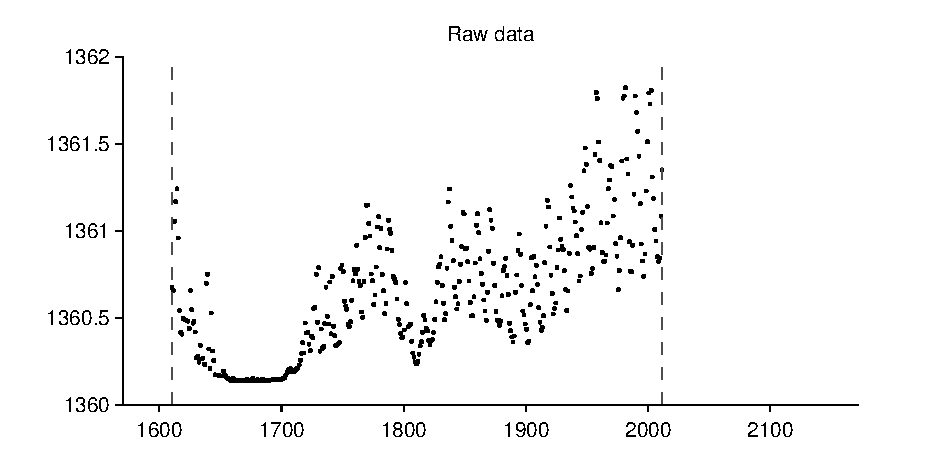
\includegraphics[width=\wmgd,height=\hmgd]{\mdrd/02-solar_raw_data} & 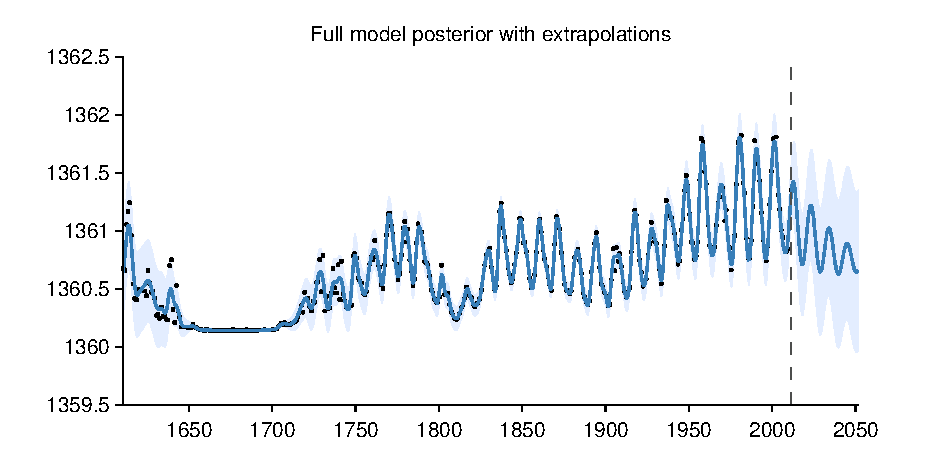
\includegraphics[width=\wmgd,height=\hmgd]{\mdrd/02-solar_all}
\end{tabular}
\caption{Raw data (left) and model posterior with extrapolation (right)}
\label{fig:rawandfit}
\end{figure}

The structure search algorithm has identified nine additive components in the data.
The  first 4 additive components explain 92.3\% of the variation in the data as shown by the coefficient of determination ($R^2$) values in table~\ref{table:stats}.
The  first 8 additive components explain 99.2\% of the variation in the data.
After the first 5 components the cross validated mean absolute error (MAE) does not decrease by more than 0.1\%.
This suggests that subsequent terms are modelling very short term trends, uncorrelated noise or are artefacts of the model or search procedure.
Short summaries of the additive components are as follows:
\begin{itemize}

  \item A constant. 

  \item A constant. This function applies from 1644 until 1713.
 

  \item A smooth function. This function applies until 1643 and from 1716 onwards. 

  \item An approximately periodic function with a period of 10.8 years. This function applies until 1643 and from 1716 onwards. 

  \item A rapidly varying smooth function. This function applies until 1643 and from 1716 onwards. 

  \item Uncorrelated noise with standard deviation increasing linearly away from 1837. This function applies until 1643 and from 1716 onwards. 

  \item Uncorrelated noise with standard deviation increasing linearly away from 1952. This function applies until 1643 and from 1716 onwards. 

  \item A rapidly varying smooth function. This function applies until 1644 and from 1719 until 1751.
 

  \item A constant. This function applies from 1713 until 1719. 

\end{itemize}

\begin{table}[htb]
\begin{center}
{\small
\begin{tabular}{|r|rrrrr|}
\hline
\bf{\#} & {$R^2$ (\%)} & {$\Delta R^2$ (\%)} & {Residual $R^2$ (\%)} & {Cross validated MAE} & Reduction in MAE (\%)\\
\hline
- & - & - & - & 1360.65 & -\\

1 & 0.0 & 0.0 & 0.0 & 0.33 & 100.0\\

2 & 35.3 & 35.3 & 35.3 & 0.23 & 29.4\\

3 & 72.5 & 37.2 & 57.5 & 0.18 & 20.7\\

4 & 92.3 & 19.9 & 72.2 & 0.15 & 16.4\\

5 & 97.8 & 5.5 & 71.4 & 0.15 & 0.4\\

6 & 97.8 & 0.0 & 0.2 & 0.15 & 0.0\\

7 & 98.4 & 0.5 & 24.8 & 0.15 & -0.0\\

8 & 99.2 & 0.8 & 50.7 & 0.15 & -0.0\\

9 & 100.0 & 0.8 & 100.0 & 0.15 & -0.0\\

\hline
\end{tabular}
\caption{
Summary statistics for cumulative additive fits to the data.
The residual coefficient of determination ($R^2$) values are computed using the residuals from the previous fit as the target values; this measures how much of the residual variance is explained by each new component.
The mean absolute error (MAE) is calculated using 10 fold cross validation with a contiguous block design; this measures the ability of the model to interpolate and extrapolate over moderate distances.
The model is fit using the full data so the MAE values cannot be used reliably as an estimate of out-of-sample predictive performance.
}
\label{table:stats}
}
\end{center}
\end{table}

\section{Detailed discussion of additive components}

\subsection{Component 1 : A constant}

This component is constant.

This component explains 0.0\% of the total variance.
The addition of this component reduces the cross validated MAE by 100.0\% from 1360.6 to 0.3.


\begin{figure}[H]
\newcommand{\wmgd}{0.5\columnwidth}
\newcommand{\hmgd}{3.0cm}
\newcommand{\mdrd}{figures/02-solar}
\newcommand{\mbm}{\hspace{-0.3cm}}
\begin{tabular}{cc}
\mbm 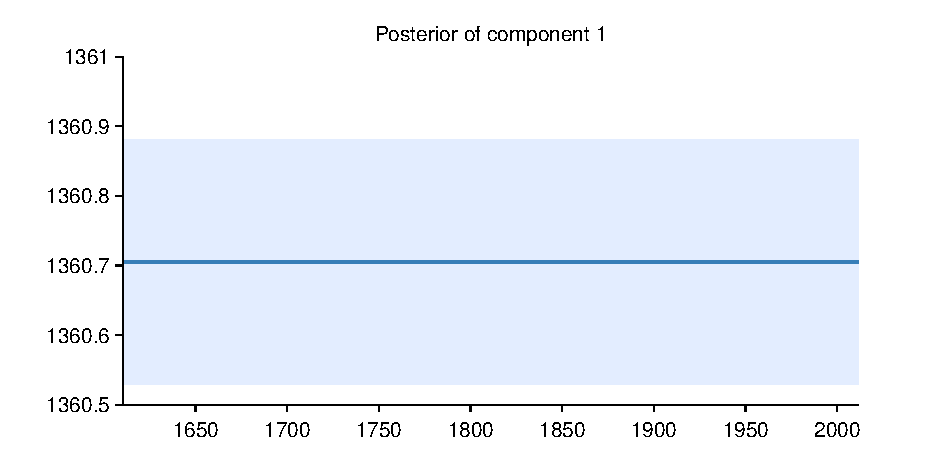
\includegraphics[width=\wmgd,height=\hmgd]{\mdrd/02-solar_1} & 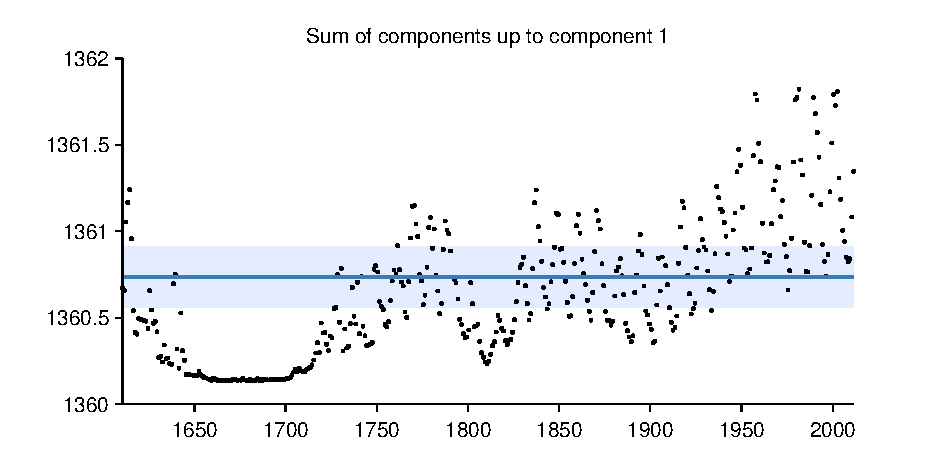
\includegraphics[width=\wmgd,height=\hmgd]{\mdrd/02-solar_1_cum}
\end{tabular}
\caption{Posterior of component 1 (left) and the posterior of the cumulative sum of components with data (right)}
\label{fig:comp1}
\end{figure}

\subsection{Component 2 : A constant. This function applies from 1644 until 1713}

This component is constant.
This component applies from 1644 until 1713.

This component explains 35.3\% of the residual variance; this increases the total variance explained from 0.0\% to 35.3\%.
The addition of this component reduces the cross validated MAE by 29.42\% from 0.33 to 0.23.


\begin{figure}[H]
\newcommand{\wmgd}{0.5\columnwidth}
\newcommand{\hmgd}{3.0cm}
\newcommand{\mdrd}{figures/02-solar}
\newcommand{\mbm}{\hspace{-0.3cm}}
\begin{tabular}{cc}
\mbm 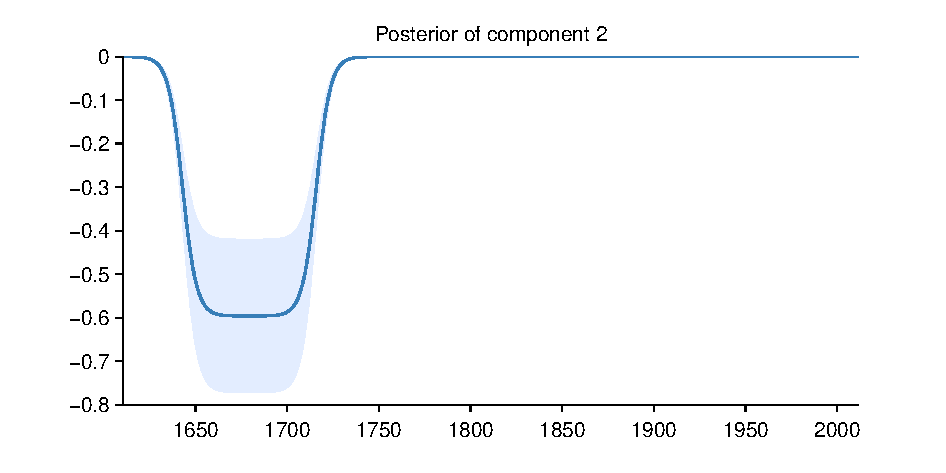
\includegraphics[width=\wmgd,height=\hmgd]{\mdrd/02-solar_2} & 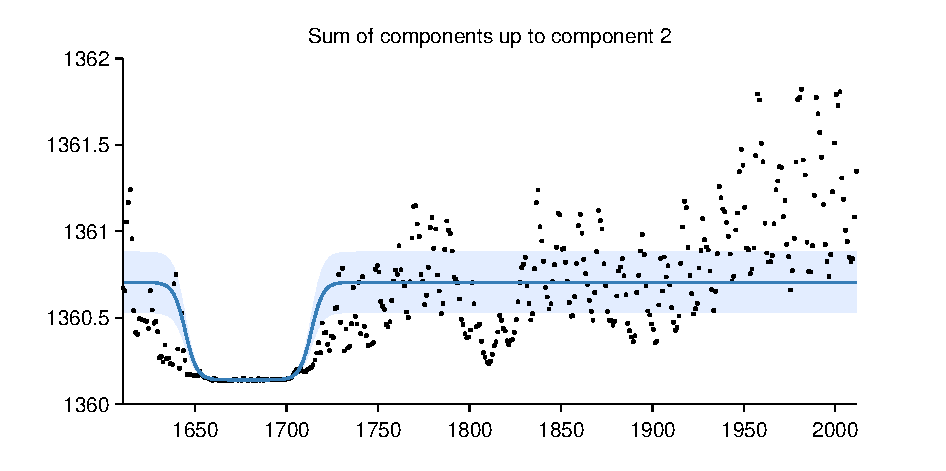
\includegraphics[width=\wmgd,height=\hmgd]{\mdrd/02-solar_2_cum}
\end{tabular}
\caption{Posterior of component 2 (left) and the posterior of the cumulative sum of components with data (right)}
\label{fig:comp2}
\end{figure}

\subsection{Component 3 : A smooth function. This function applies until 1644 and from 1719 onwards}

This component is a smooth function with a typical lengthscale of 23.1 years.
This component applies until 1643 and from 1716 onwards.

This component explains 57.5\% of the residual variance; this increases the total variance explained from 35.3\% to 72.5\%.
The addition of this component reduces the cross validated MAE by 20.66\% from 0.23 to 0.18.


\begin{figure}[H]
\newcommand{\wmgd}{0.5\columnwidth}
\newcommand{\hmgd}{3.0cm}
\newcommand{\mdrd}{figures/02-solar}
\newcommand{\mbm}{\hspace{-0.3cm}}
\begin{tabular}{cc}
\mbm 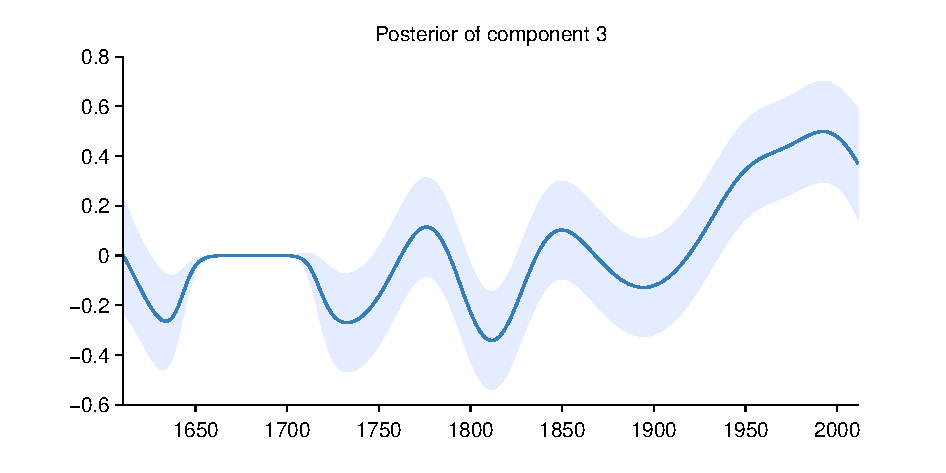
\includegraphics[width=\wmgd,height=\hmgd]{\mdrd/02-solar_3} & 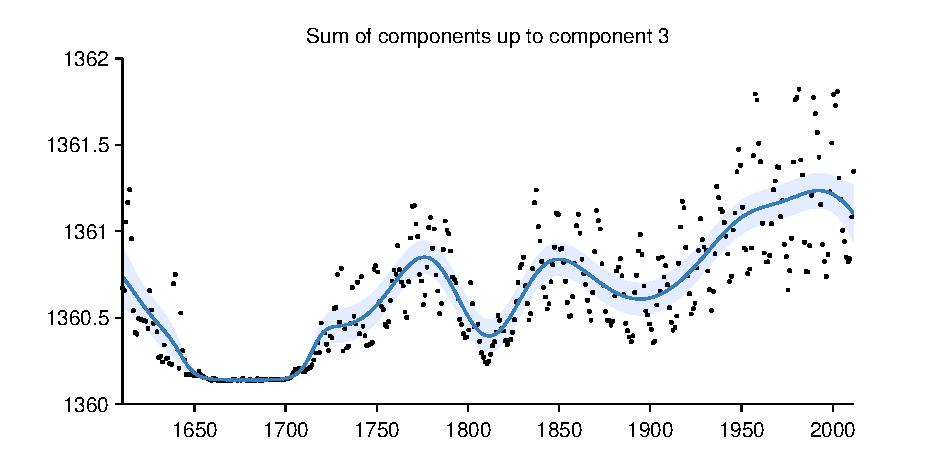
\includegraphics[width=\wmgd,height=\hmgd]{\mdrd/02-solar_3_cum}
\end{tabular}
\caption{Posterior of component 3 (left) and the posterior of the cumulative sum of components with data (right)}
\label{fig:comp3}
\end{figure}

\subsection{Component 4 : An approximately periodic function with a period of 10.8 years. This function applies until 1644 and from 1719 onwards}

This component is approximately periodic with a period of 10.8 years.
Across periods the shape of this function varies smoothly with a typical lengthscale of 36.9 years.
The shape of this function within each period is very smooth and resembles a sinusoid.
This component applies until 1643 and from 1716 onwards.

This component explains 72.2\% of the residual variance; this increases the total variance explained from 72.5\% to 92.3\%.
The addition of this component reduces the cross validated MAE by 16.42\% from 0.18 to 0.15.


\begin{figure}[H]
\newcommand{\wmgd}{0.5\columnwidth}
\newcommand{\hmgd}{3.0cm}
\newcommand{\mdrd}{figures/02-solar}
\newcommand{\mbm}{\hspace{-0.3cm}}
\begin{tabular}{cc}
\mbm 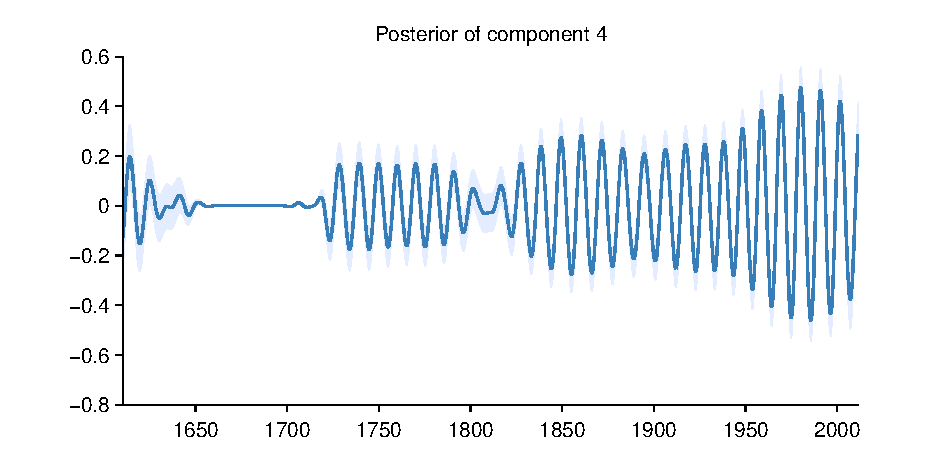
\includegraphics[width=\wmgd,height=\hmgd]{\mdrd/02-solar_4} & 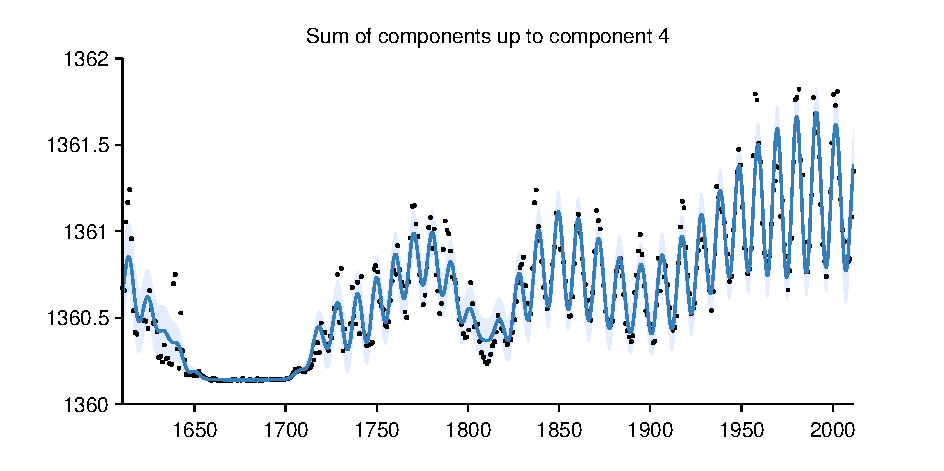
\includegraphics[width=\wmgd,height=\hmgd]{\mdrd/02-solar_4_cum}
\end{tabular}
\caption{Posterior of component 4 (left) and the posterior of the cumulative sum of components with data (right)}
\label{fig:comp4}
\end{figure}

\subsection{Component 5 : A rapidly varying smooth function. This function applies until 1644 and from 1719 onwards}

This component is a rapidly varying but smooth function with a typical lengthscale of 1.6 years.
This component applies until 1643 and from 1716 onwards.

This component explains 71.4\% of the residual variance; this increases the total variance explained from 92.3\% to 97.8\%.
The addition of this component reduces the cross validated MAE by 0.41\% from 0.15 to 0.15.


\begin{figure}[H]
\newcommand{\wmgd}{0.5\columnwidth}
\newcommand{\hmgd}{3.0cm}
\newcommand{\mdrd}{figures/02-solar}
\newcommand{\mbm}{\hspace{-0.3cm}}
\begin{tabular}{cc}
\mbm 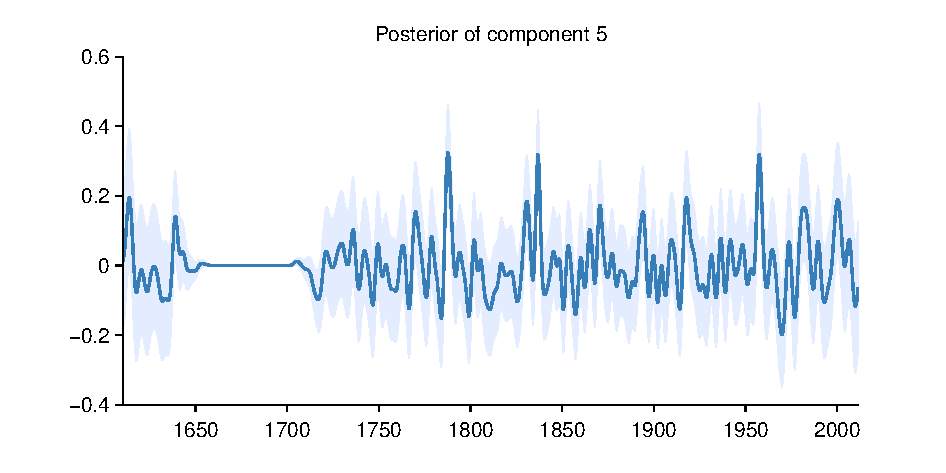
\includegraphics[width=\wmgd,height=\hmgd]{\mdrd/02-solar_5} & 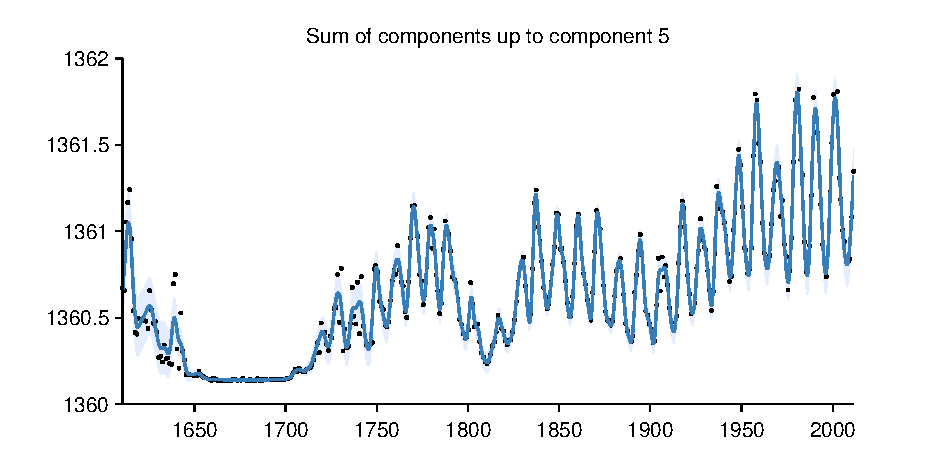
\includegraphics[width=\wmgd,height=\hmgd]{\mdrd/02-solar_5_cum}
\end{tabular}
\caption{Posterior of component 5 (left) and the posterior of the cumulative sum of components with data (right)}
\label{fig:comp5}
\end{figure}

\subsection{Component 6 : Uncorrelated noise}

This component models uncorrelated noise.
The standard deviation of the noise increases linearly away from 1837.
This component applies until 1643 and from 1716 onwards.

This component explains 0.2\% of the residual variance; this increases the total variance explained from 97.8\% to 97.8\%.
The addition of this component reduces the cross validated MAE by 0.00\% from 0.15 to 0.15.
This component explains residual variance but does not improve MAE which suggests that this component describes very short term patterns, uncorrelated noise or is an artefact of the model or search procedure.

\begin{figure}[H]
\newcommand{\wmgd}{0.5\columnwidth}
\newcommand{\hmgd}{3.0cm}
\newcommand{\mdrd}{figures/02-solar}
\newcommand{\mbm}{\hspace{-0.3cm}}
\begin{tabular}{cc}
\mbm 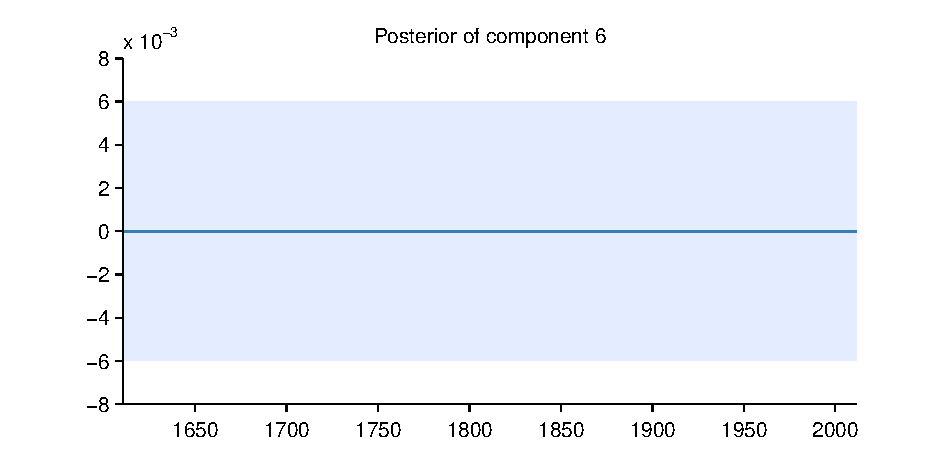
\includegraphics[width=\wmgd,height=\hmgd]{\mdrd/02-solar_6} & 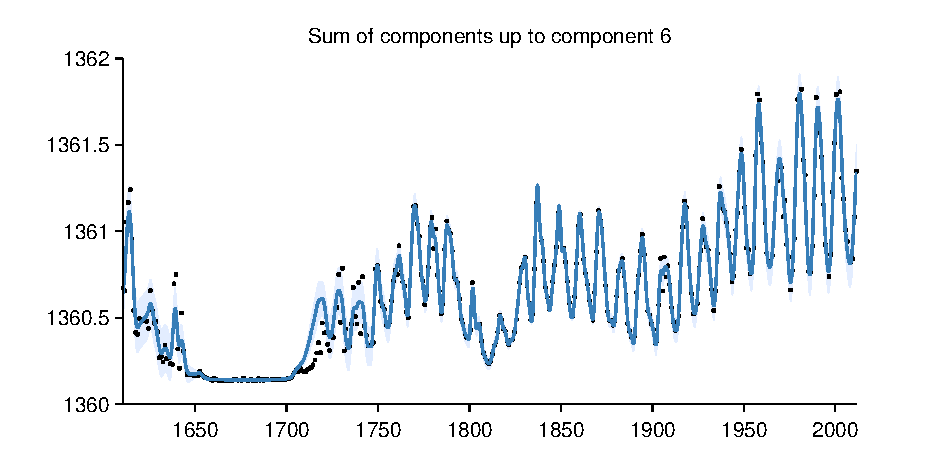
\includegraphics[width=\wmgd,height=\hmgd]{\mdrd/02-solar_6_cum}
\end{tabular}
\caption{Posterior of component 6 (left) and the posterior of the cumulative sum of components with data (right)}
\label{fig:comp6}
\end{figure}

\subsection{Component 7 : A rapidly varying smooth function with marginal standard deviation increasing linearly away from 1843. This function applies from 1751 onwards}

This function is a rapidly varying but smooth function with a typical lengthscale of 3.1 months.
The marginal standard deviation of the function increases linearly away from 1843.
This component applies from 1751 onwards.

This component explains 24.8\% of the residual variance; this increases the total variance explained from 97.8\% to 98.4\%.
The addition of this component increases the cross validated MAE by 0.00\% from 0.15 to 0.15.
This component explains residual variance but does not improve MAE which suggests that this component describes very short term patterns, uncorrelated noise or is an artefact of the model or search procedure.

\begin{figure}[H]
\newcommand{\wmgd}{0.5\columnwidth}
\newcommand{\hmgd}{3.0cm}
\newcommand{\mdrd}{figures/02-solar}
\newcommand{\mbm}{\hspace{-0.3cm}}
\begin{tabular}{cc}
\mbm 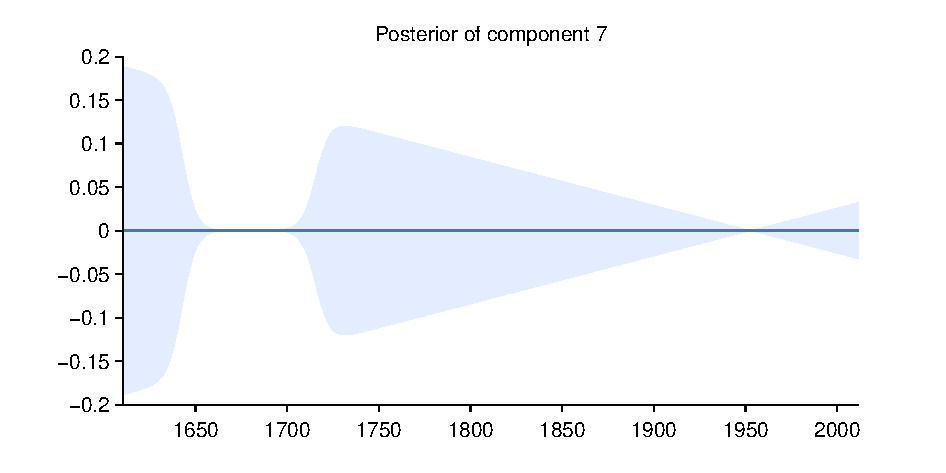
\includegraphics[width=\wmgd,height=\hmgd]{\mdrd/02-solar_7} & 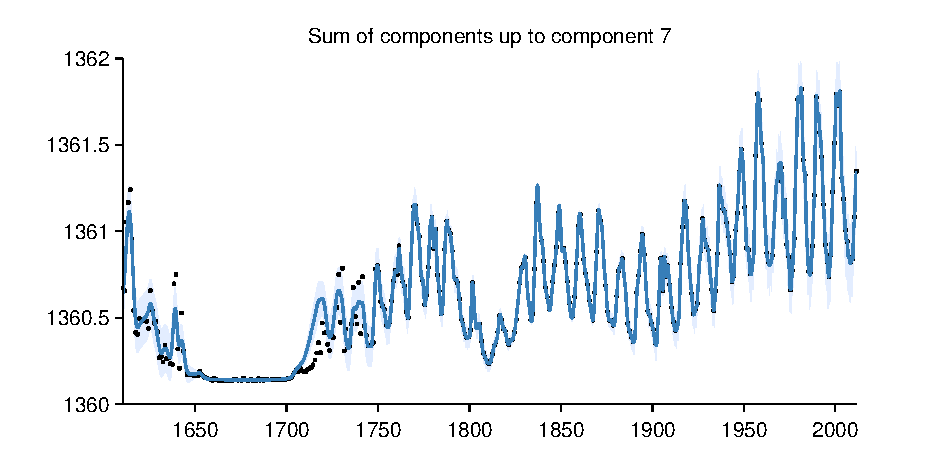
\includegraphics[width=\wmgd,height=\hmgd]{\mdrd/02-solar_7_cum}
\end{tabular}
\caption{Posterior of component 7 (left) and the posterior of the cumulative sum of components with data (right)}
\label{fig:comp7}
\end{figure}

\subsection{Component 8 : A rapidly varying smooth function. This function applies until 1644 and from 1719 until 1751}

This function is a rapidly varying but smooth function with a typical lengthscale of 3.1 months.
This component applies until 1644 and from 1719 until 1751.

This component explains 50.7\% of the residual variance; this increases the total variance explained from 98.4\% to 99.2\%.
The addition of this component increases the cross validated MAE by 0.00\% from 0.15 to 0.15.
This component explains residual variance but does not improve MAE which suggests that this component describes very short term patterns, uncorrelated noise or is an artefact of the model or search procedure.

\begin{figure}[H]
\newcommand{\wmgd}{0.5\columnwidth}
\newcommand{\hmgd}{3.0cm}
\newcommand{\mdrd}{figures/02-solar}
\newcommand{\mbm}{\hspace{-0.3cm}}
\begin{tabular}{cc}
\mbm 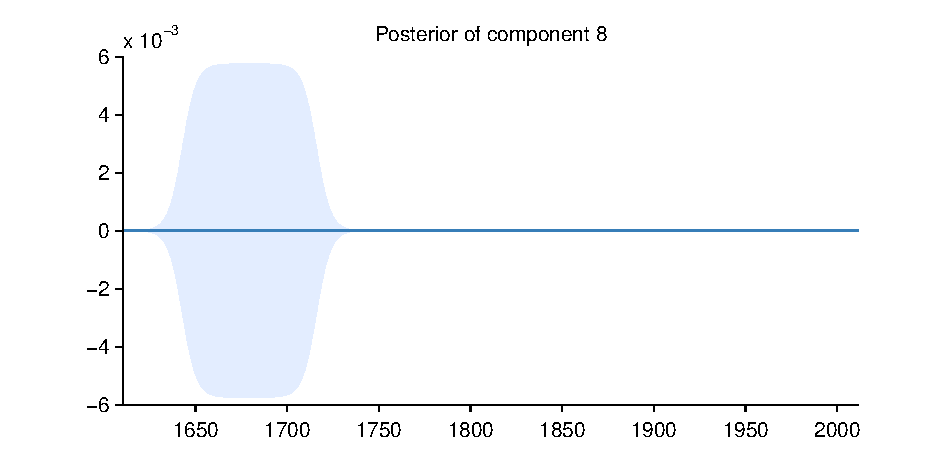
\includegraphics[width=\wmgd,height=\hmgd]{\mdrd/02-solar_8} & 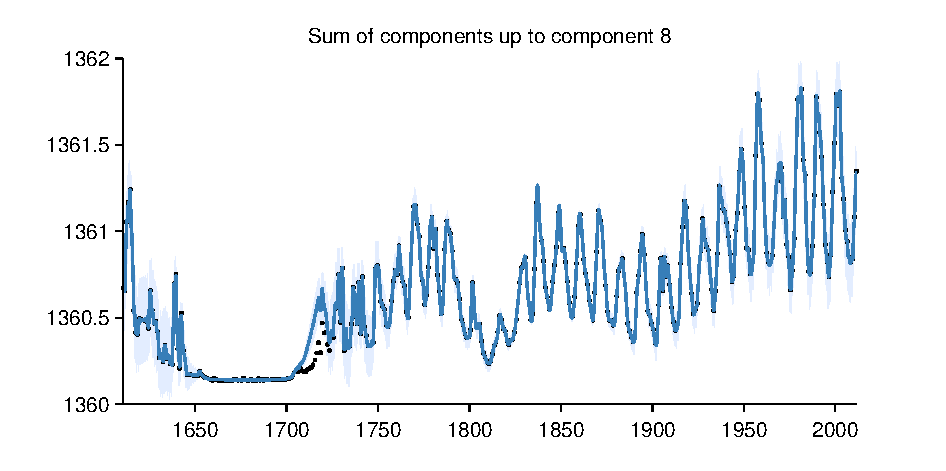
\includegraphics[width=\wmgd,height=\hmgd]{\mdrd/02-solar_8_cum}
\end{tabular}
\caption{Posterior of component 8 (left) and the posterior of the cumulative sum of components with data (right)}
\label{fig:comp8}
\end{figure}

\subsection{Component 9 : A constant. This function applies from 1713 until 1719}

This component is constant.
This component applies from 1713 until 1719.

This component explains 100.0\% of the residual variance; this increases the total variance explained from 99.2\% to 100.0\%.
The addition of this component increases the cross validated MAE by 0.01\% from 0.15 to 0.15.
This component explains residual variance but does not improve MAE which suggests that this component describes very short term patterns, uncorrelated noise or is an artefact of the model or search procedure.

\begin{figure}[H]
\newcommand{\wmgd}{0.5\columnwidth}
\newcommand{\hmgd}{3.0cm}
\newcommand{\mdrd}{figures/02-solar}
\newcommand{\mbm}{\hspace{-0.3cm}}
\begin{tabular}{cc}
\mbm 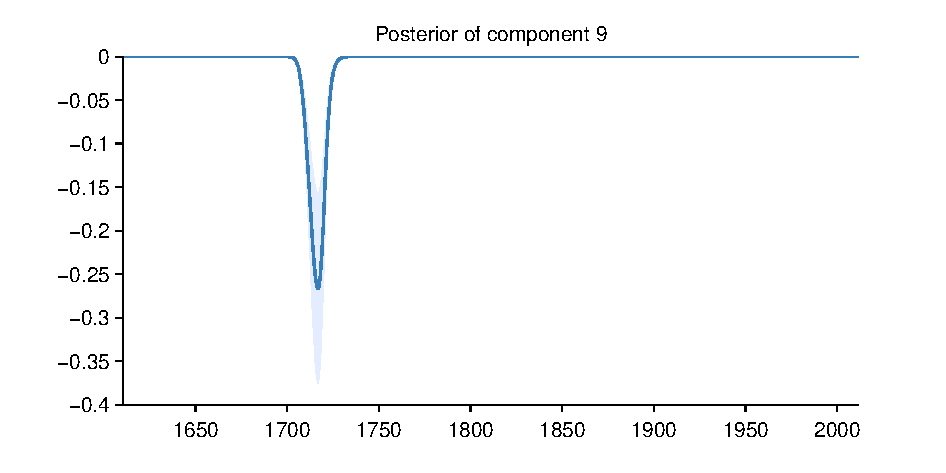
\includegraphics[width=\wmgd,height=\hmgd]{\mdrd/02-solar_9} & 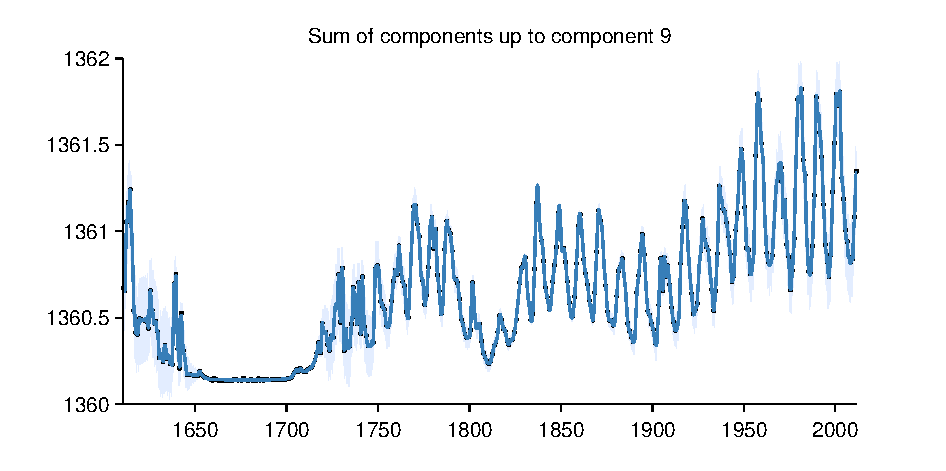
\includegraphics[width=\wmgd,height=\hmgd]{\mdrd/02-solar_9_cum}
\end{tabular}
\caption{Posterior of component 9 (left) and the posterior of the cumulative sum of components with data (right)}
\label{fig:comp9}
\end{figure}

\section{Extrapolation}

Summaries of the posterior distribution of the full model are shown in figure~\ref{fig:extrap}.
The plot on the left displays the mean of the posterior together with pointwise variance.
The plot on the right displays three random samples from the posterior.

\begin{figure}[H]
\newcommand{\wmgd}{0.5\columnwidth}
\newcommand{\hmgd}{3.0cm}
\newcommand{\mdrd}{figures/02-solar}
\newcommand{\mbm}{\hspace{-0.3cm}}
\begin{tabular}{cc}
\mbm 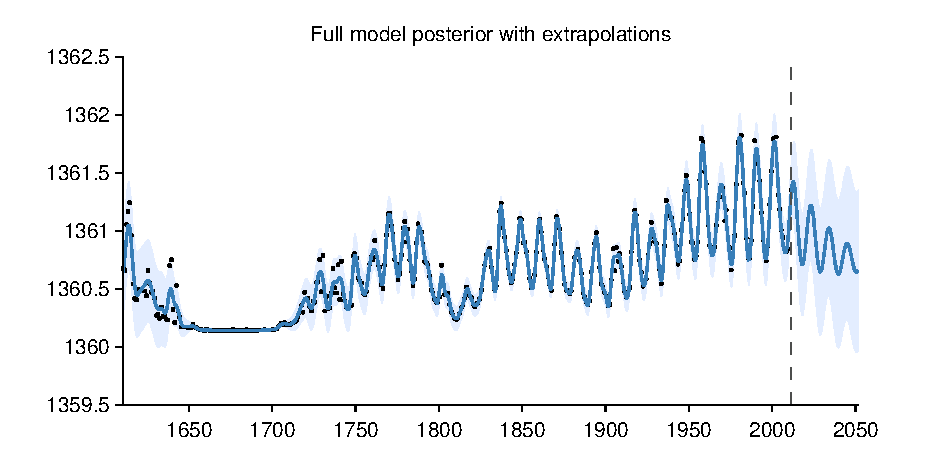
\includegraphics[width=\wmgd,height=\hmgd]{\mdrd/02-solar_all} & 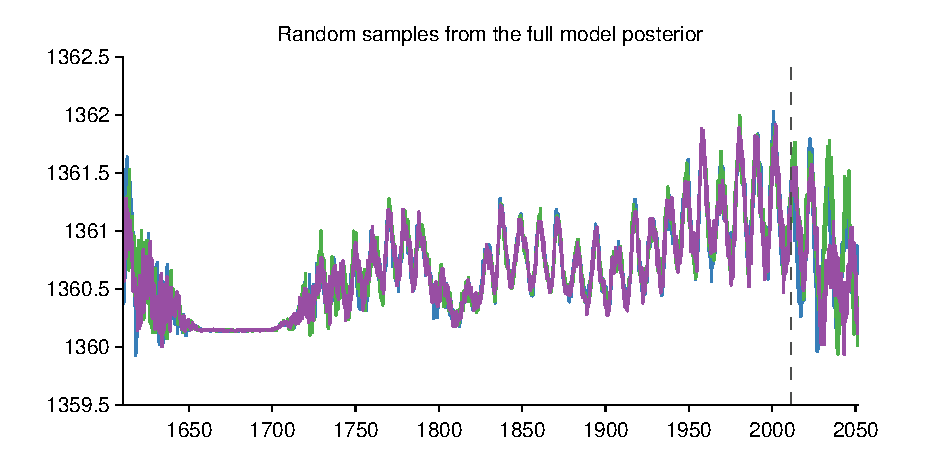
\includegraphics[width=\wmgd,height=\hmgd]{\mdrd/02-solar_all_sample}
\end{tabular}
\caption{Full model posterior. Mean and pointwise variance (left) and three random samples (right)}
\label{fig:extrap}
\end{figure}

\subsection{Component 1 : A constant}

Some discussion about extrapolation.

\begin{figure}[H]
\newcommand{\wmgd}{0.5\columnwidth}
\newcommand{\hmgd}{3.0cm}
\newcommand{\mdrd}{figures/02-solar}
\newcommand{\mbm}{\hspace{-0.3cm}}
\begin{tabular}{cc}
\mbm 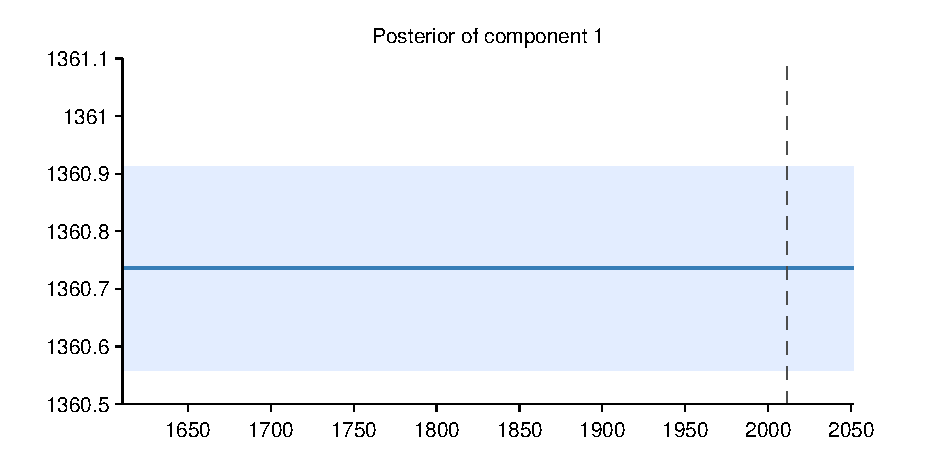
\includegraphics[width=\wmgd,height=\hmgd]{\mdrd/02-solar_1_extrap} & 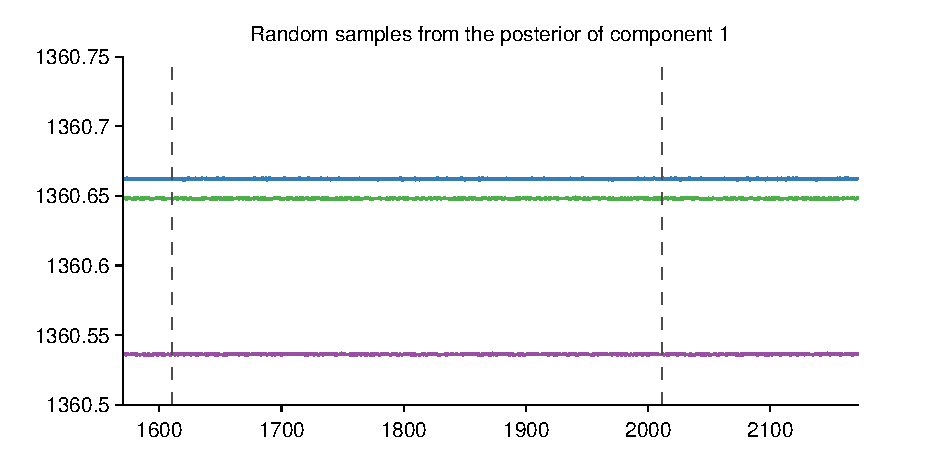
\includegraphics[width=\wmgd,height=\hmgd]{\mdrd/02-solar_1_sample} \\
\mbm 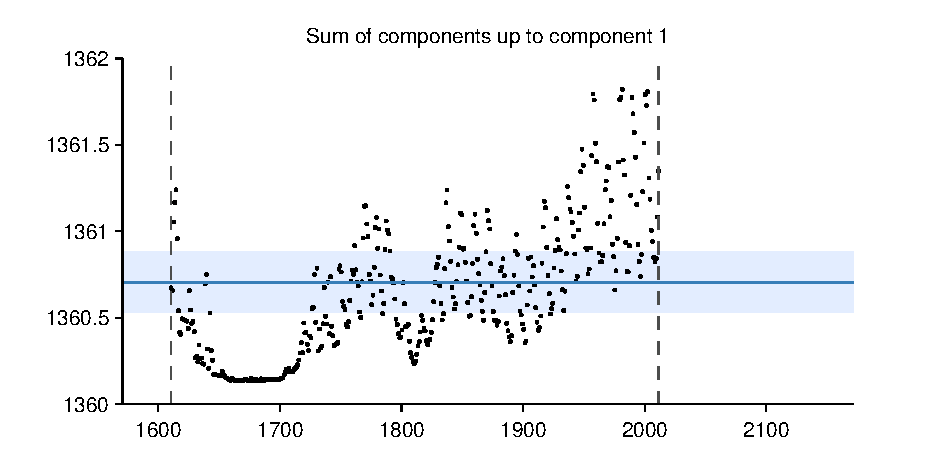
\includegraphics[width=\wmgd,height=\hmgd]{\mdrd/02-solar_1_cum_extrap} & 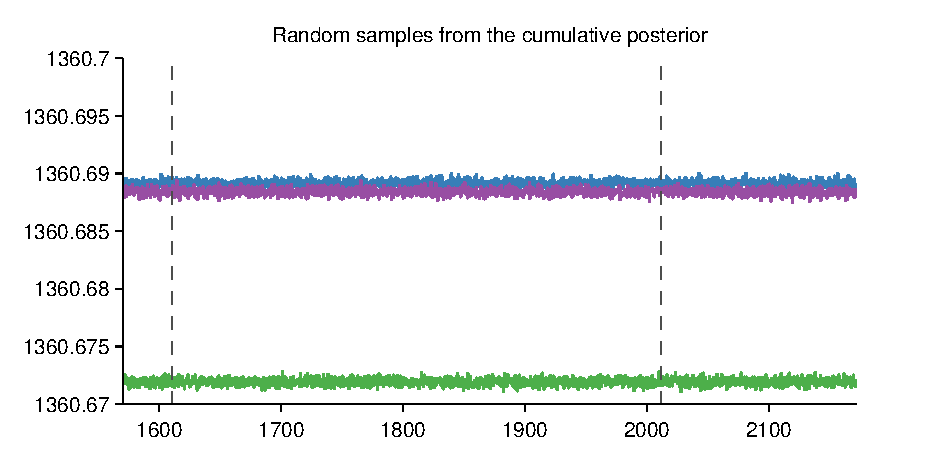
\includegraphics[width=\wmgd,height=\hmgd]{\mdrd/02-solar_1_cum_sample}
\end{tabular}
\caption{Posterior of component 1. Mean and pointwise variance (left) and three random samples from this distribution (right)}
\label{fig:extrap1}
\end{figure}

\subsection{Component 2 : A constant. This function applies from 1644 until 1713}

Some discussion about extrapolation.

\begin{figure}[H]
\newcommand{\wmgd}{0.5\columnwidth}
\newcommand{\hmgd}{3.0cm}
\newcommand{\mdrd}{figures/02-solar}
\newcommand{\mbm}{\hspace{-0.3cm}}
\begin{tabular}{cc}
\mbm 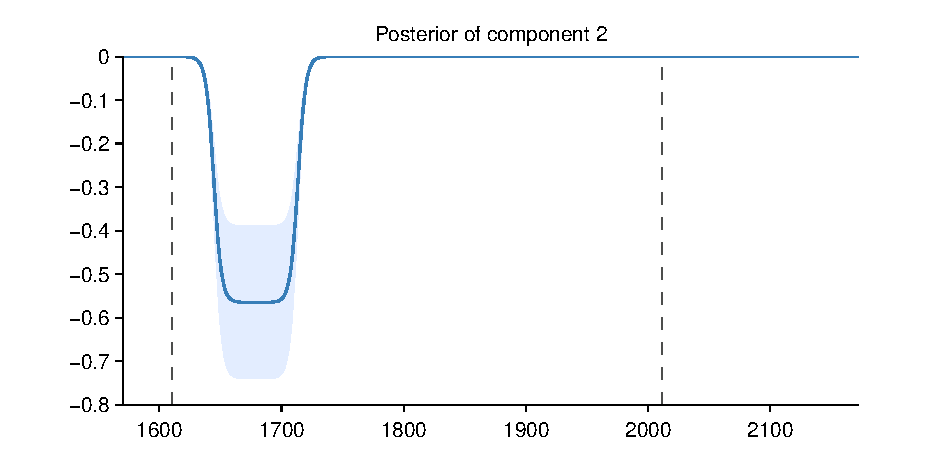
\includegraphics[width=\wmgd,height=\hmgd]{\mdrd/02-solar_2_extrap} & 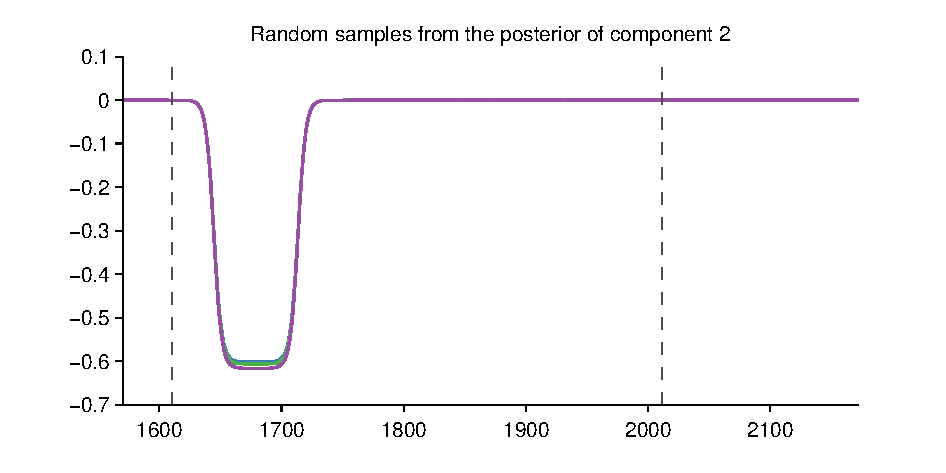
\includegraphics[width=\wmgd,height=\hmgd]{\mdrd/02-solar_2_sample} \\
\mbm 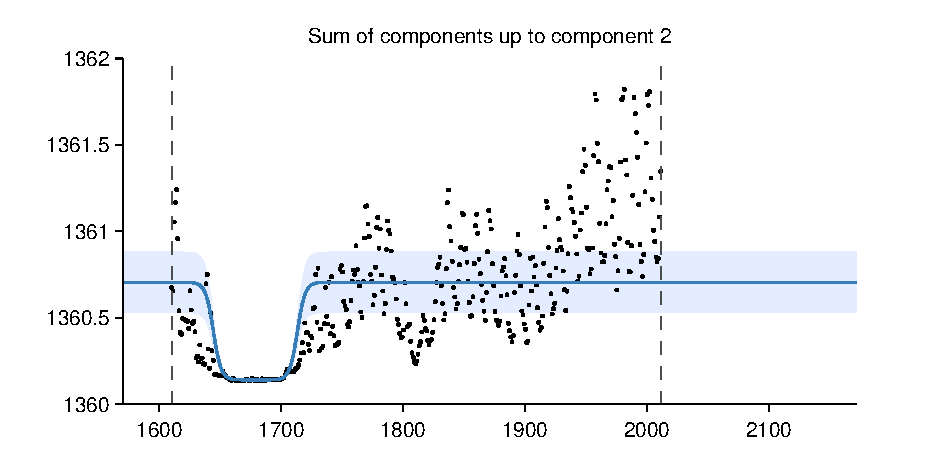
\includegraphics[width=\wmgd,height=\hmgd]{\mdrd/02-solar_2_cum_extrap} & 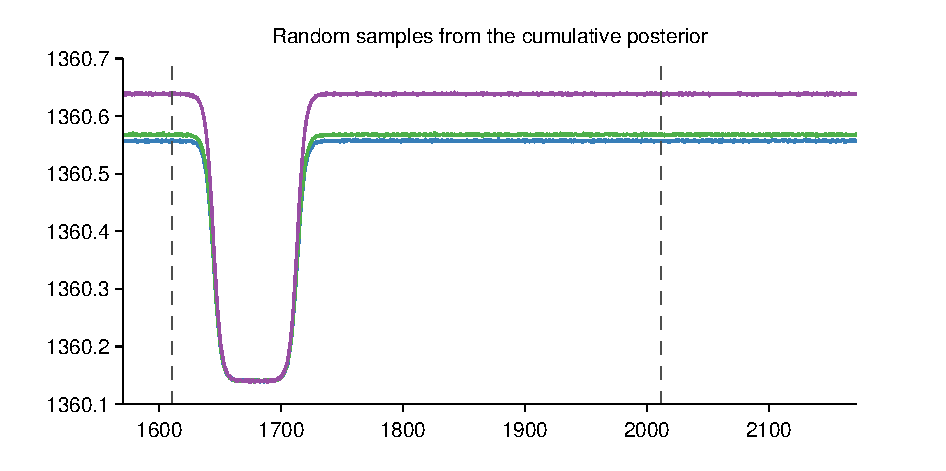
\includegraphics[width=\wmgd,height=\hmgd]{\mdrd/02-solar_2_cum_sample}
\end{tabular}
\caption{Posterior of component 2. Mean and pointwise variance (left) and three random samples from this distribution (right)}
\label{fig:extrap2}
\end{figure}

\subsection{Component 3 : A smooth function. This function applies until 1644 and from 1719 onwards}

Some discussion about extrapolation.

\begin{figure}[H]
\newcommand{\wmgd}{0.5\columnwidth}
\newcommand{\hmgd}{3.0cm}
\newcommand{\mdrd}{figures/02-solar}
\newcommand{\mbm}{\hspace{-0.3cm}}
\begin{tabular}{cc}
\mbm 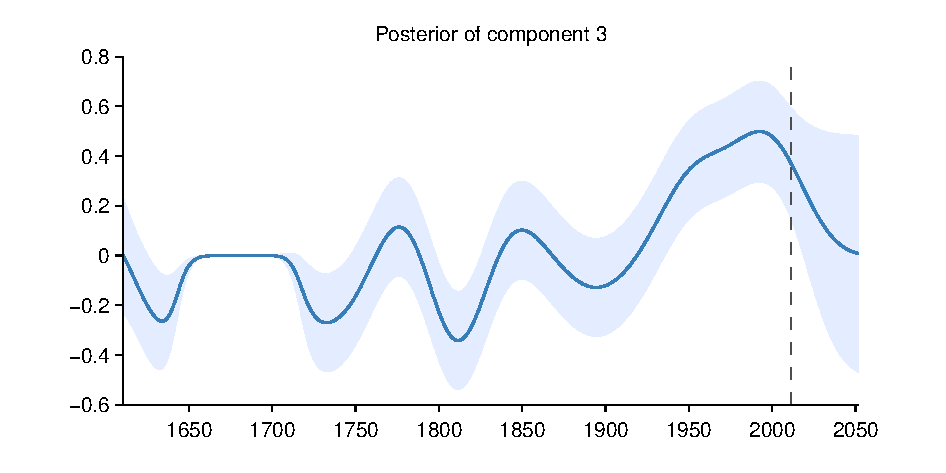
\includegraphics[width=\wmgd,height=\hmgd]{\mdrd/02-solar_3_extrap} & 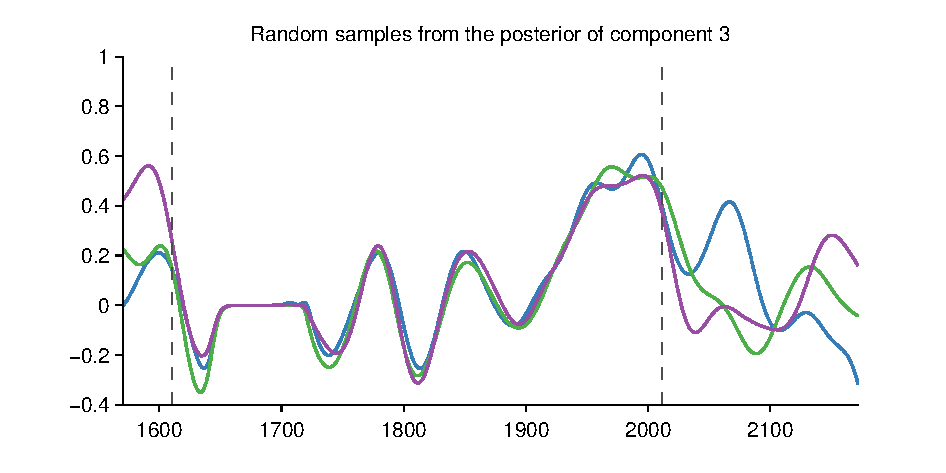
\includegraphics[width=\wmgd,height=\hmgd]{\mdrd/02-solar_3_sample} \\
\mbm 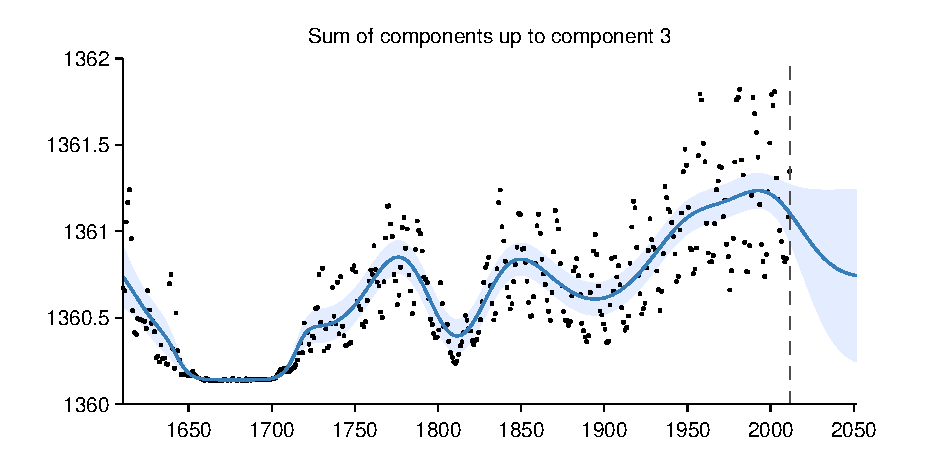
\includegraphics[width=\wmgd,height=\hmgd]{\mdrd/02-solar_3_cum_extrap} & 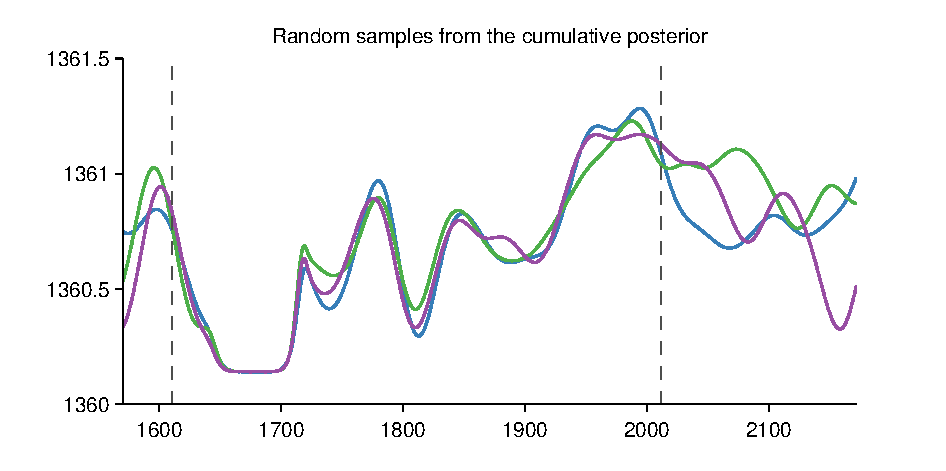
\includegraphics[width=\wmgd,height=\hmgd]{\mdrd/02-solar_3_cum_sample}
\end{tabular}
\caption{Posterior of component 3. Mean and pointwise variance (left) and three random samples from this distribution (right)}
\label{fig:extrap3}
\end{figure}

\subsection{Component 4 : An approximately periodic function with a period of 10.8 years. This function applies until 1644 and from 1719 onwards}

Some discussion about extrapolation.

\begin{figure}[H]
\newcommand{\wmgd}{0.5\columnwidth}
\newcommand{\hmgd}{3.0cm}
\newcommand{\mdrd}{figures/02-solar}
\newcommand{\mbm}{\hspace{-0.3cm}}
\begin{tabular}{cc}
\mbm 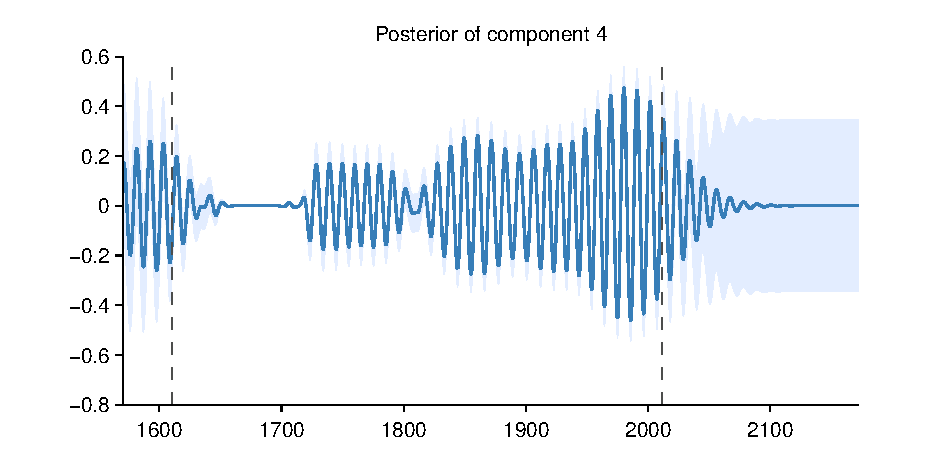
\includegraphics[width=\wmgd,height=\hmgd]{\mdrd/02-solar_4_extrap} & 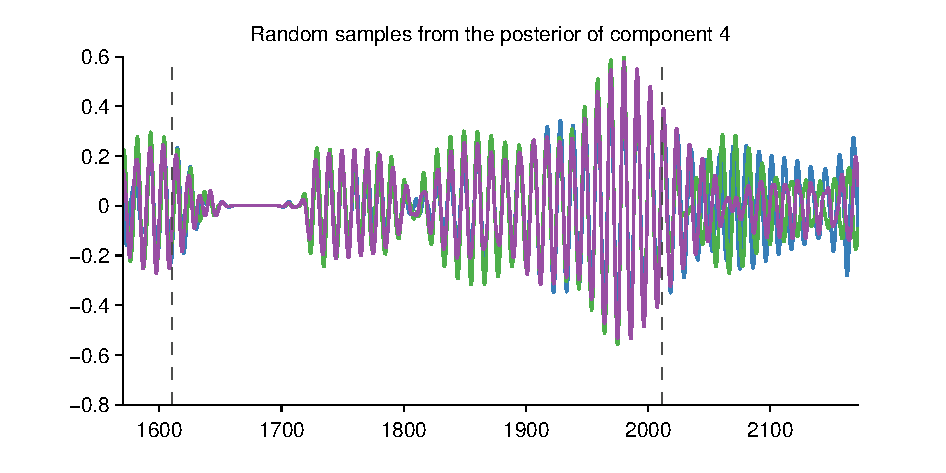
\includegraphics[width=\wmgd,height=\hmgd]{\mdrd/02-solar_4_sample} \\
\mbm 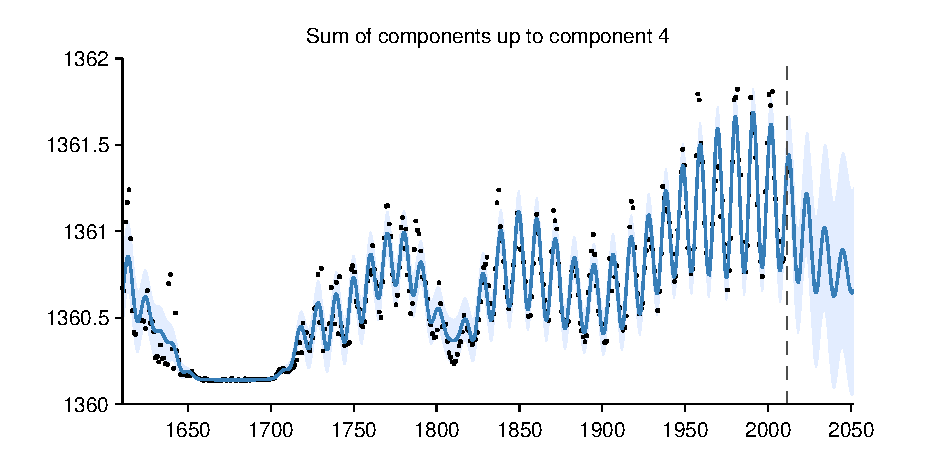
\includegraphics[width=\wmgd,height=\hmgd]{\mdrd/02-solar_4_cum_extrap} & 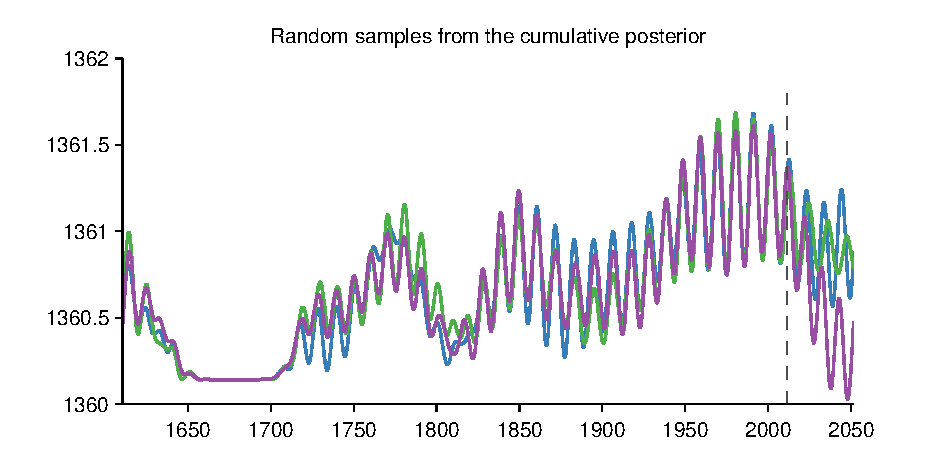
\includegraphics[width=\wmgd,height=\hmgd]{\mdrd/02-solar_4_cum_sample}
\end{tabular}
\caption{Posterior of component 4. Mean and pointwise variance (left) and three random samples from this distribution (right)}
\label{fig:extrap4}
\end{figure}

\subsection{Component 5 : A rapidly varying smooth function. This function applies until 1644 and from 1719 onwards}

Some discussion about extrapolation.

\begin{figure}[H]
\newcommand{\wmgd}{0.5\columnwidth}
\newcommand{\hmgd}{3.0cm}
\newcommand{\mdrd}{figures/02-solar}
\newcommand{\mbm}{\hspace{-0.3cm}}
\begin{tabular}{cc}
\mbm 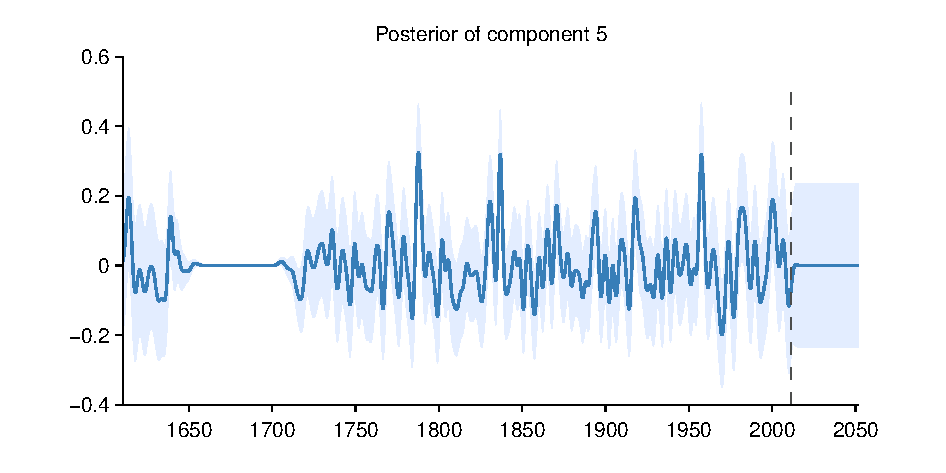
\includegraphics[width=\wmgd,height=\hmgd]{\mdrd/02-solar_5_extrap} & 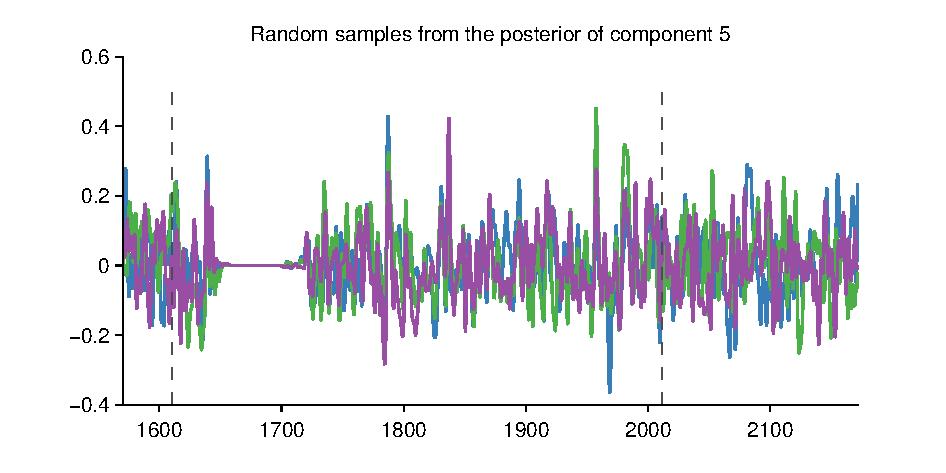
\includegraphics[width=\wmgd,height=\hmgd]{\mdrd/02-solar_5_sample} \\
\mbm 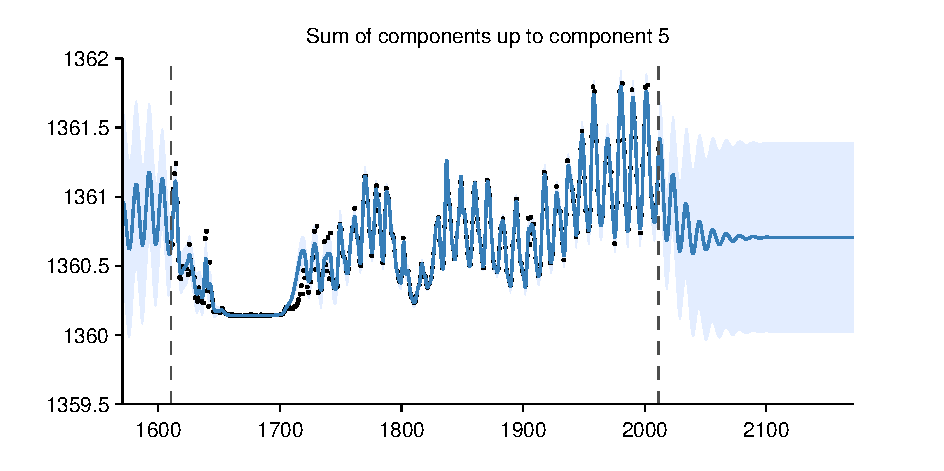
\includegraphics[width=\wmgd,height=\hmgd]{\mdrd/02-solar_5_cum_extrap} & 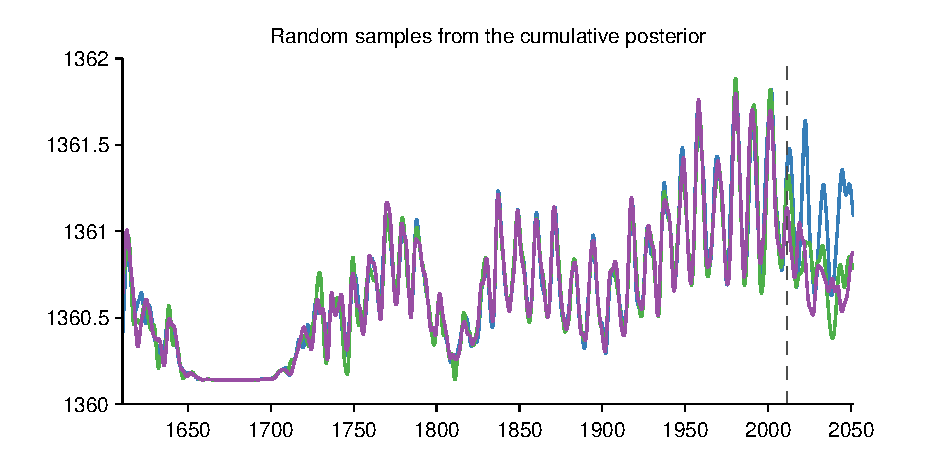
\includegraphics[width=\wmgd,height=\hmgd]{\mdrd/02-solar_5_cum_sample}
\end{tabular}
\caption{Posterior of component 5. Mean and pointwise variance (left) and three random samples from this distribution (right)}
\label{fig:extrap5}
\end{figure}

\subsection{Component 6 : Uncorrelated noise}

Some discussion about extrapolation.

\begin{figure}[H]
\newcommand{\wmgd}{0.5\columnwidth}
\newcommand{\hmgd}{3.0cm}
\newcommand{\mdrd}{figures/02-solar}
\newcommand{\mbm}{\hspace{-0.3cm}}
\begin{tabular}{cc}
\mbm 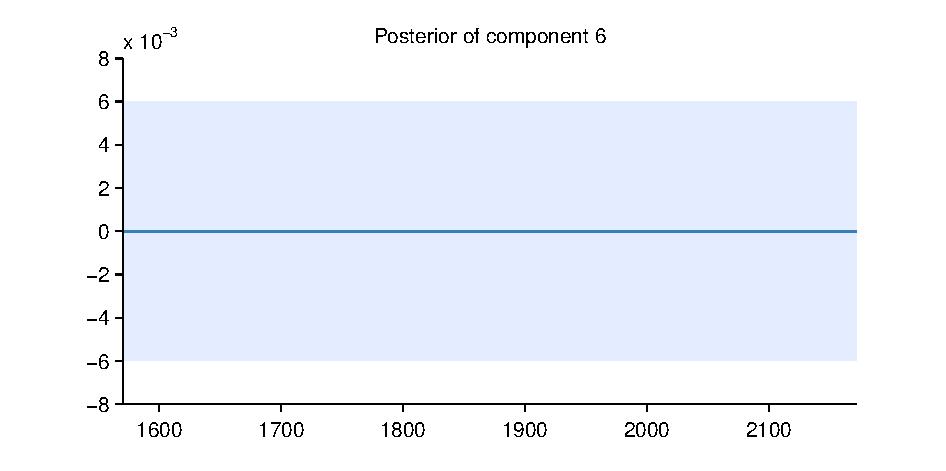
\includegraphics[width=\wmgd,height=\hmgd]{\mdrd/02-solar_6_extrap} & 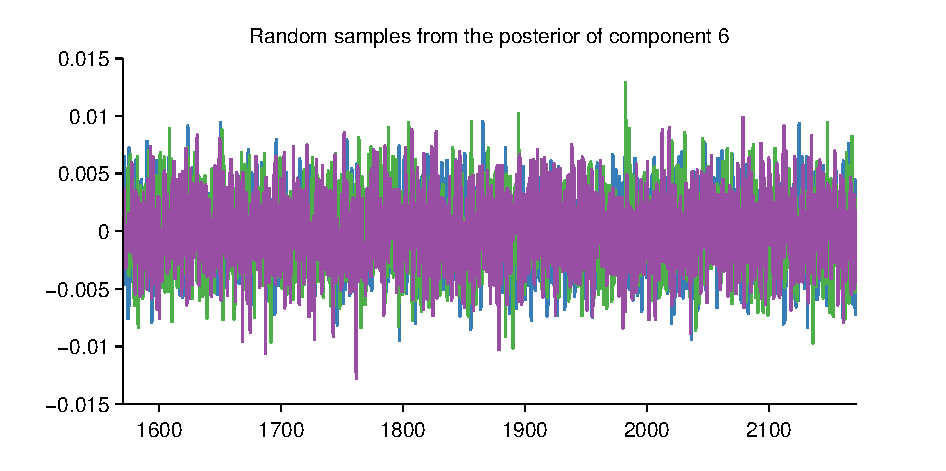
\includegraphics[width=\wmgd,height=\hmgd]{\mdrd/02-solar_6_sample} \\
\mbm 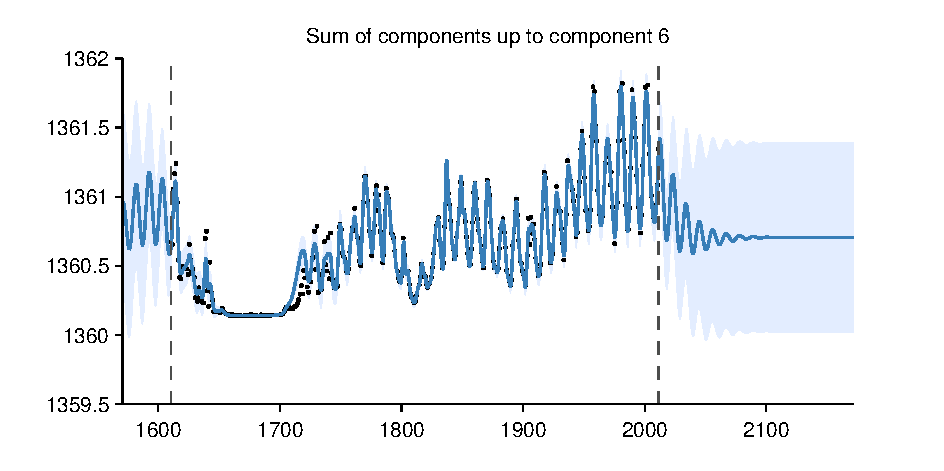
\includegraphics[width=\wmgd,height=\hmgd]{\mdrd/02-solar_6_cum_extrap} & 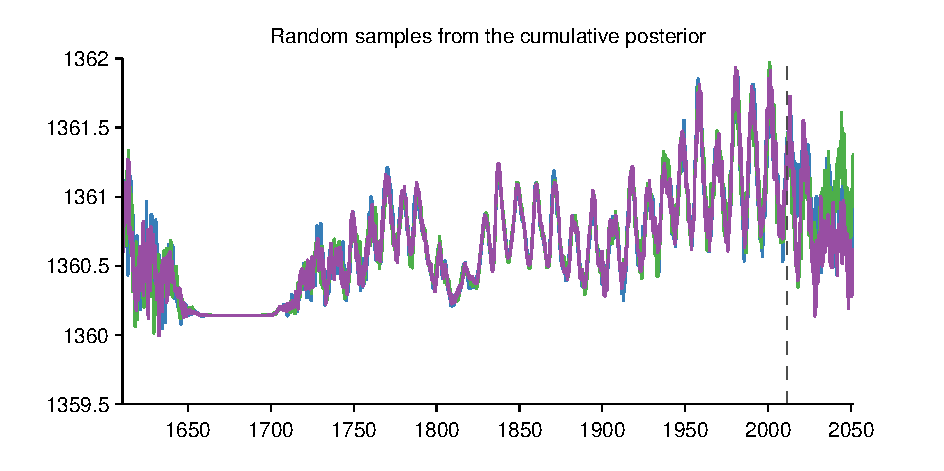
\includegraphics[width=\wmgd,height=\hmgd]{\mdrd/02-solar_6_cum_sample}
\end{tabular}
\caption{Posterior of component 6. Mean and pointwise variance (left) and three random samples from this distribution (right)}
\label{fig:extrap6}
\end{figure}

\subsection{Component 7 : A rapidly varying smooth function with marginal standard deviation increasing linearly away from 1843. This function applies from 1751 onwards}

Some discussion about extrapolation.

\begin{figure}[H]
\newcommand{\wmgd}{0.5\columnwidth}
\newcommand{\hmgd}{3.0cm}
\newcommand{\mdrd}{figures/02-solar}
\newcommand{\mbm}{\hspace{-0.3cm}}
\begin{tabular}{cc}
\mbm 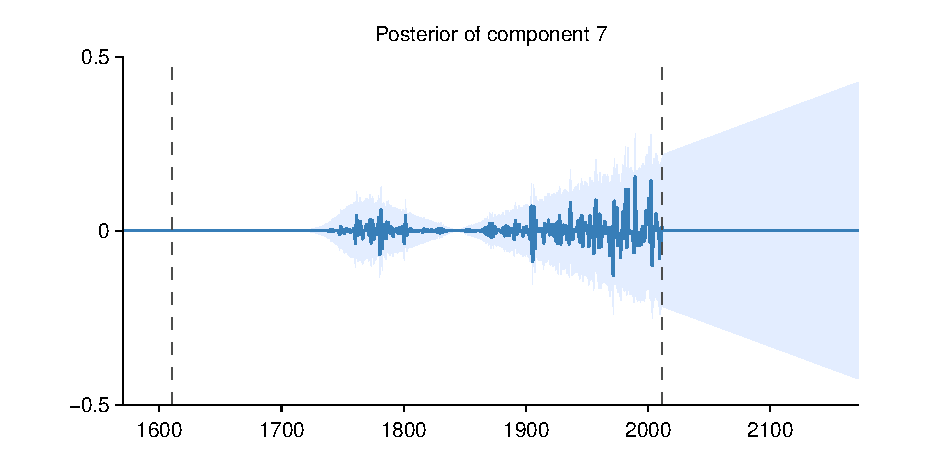
\includegraphics[width=\wmgd,height=\hmgd]{\mdrd/02-solar_7_extrap} & 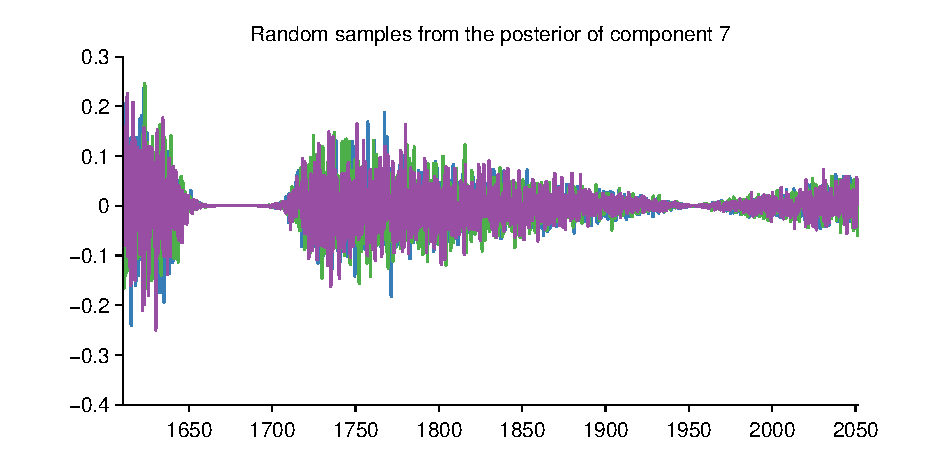
\includegraphics[width=\wmgd,height=\hmgd]{\mdrd/02-solar_7_sample} \\
\mbm 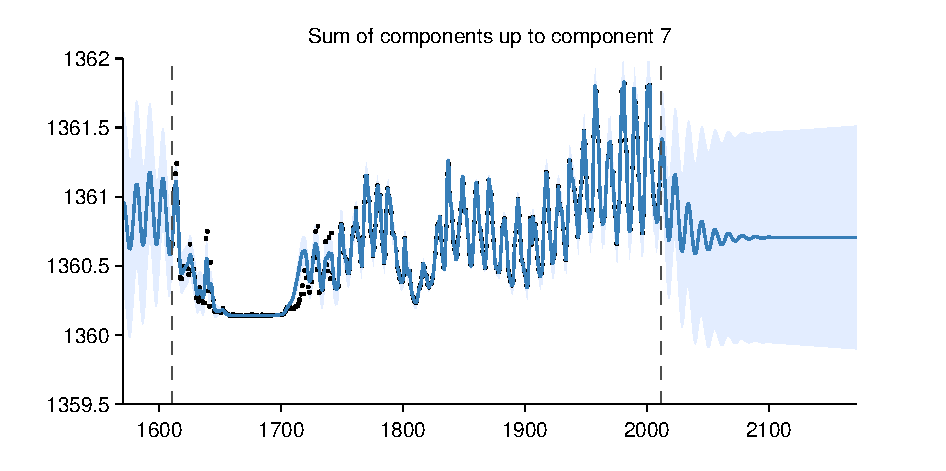
\includegraphics[width=\wmgd,height=\hmgd]{\mdrd/02-solar_7_cum_extrap} & 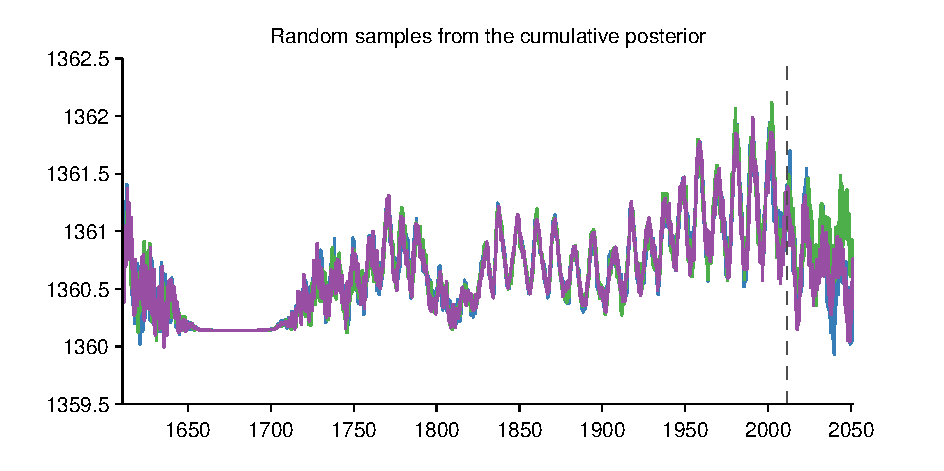
\includegraphics[width=\wmgd,height=\hmgd]{\mdrd/02-solar_7_cum_sample}
\end{tabular}
\caption{Posterior of component 7. Mean and pointwise variance (left) and three random samples from this distribution (right)}
\label{fig:extrap7}
\end{figure}

\subsection{Component 8 : A rapidly varying smooth function. This function applies until 1644 and from 1719 until 1751}

Some discussion about extrapolation.

\begin{figure}[H]
\newcommand{\wmgd}{0.5\columnwidth}
\newcommand{\hmgd}{3.0cm}
\newcommand{\mdrd}{figures/02-solar}
\newcommand{\mbm}{\hspace{-0.3cm}}
\begin{tabular}{cc}
\mbm \includegraphics[width=\wmgd,height=\hmgd]{\mdrd/02-solar_8_extrap} & \includegraphics[width=\wmgd,height=\hmgd]{\mdrd/02-solar_8_sample} \\
\mbm \includegraphics[width=\wmgd,height=\hmgd]{\mdrd/02-solar_8_cum_extrap} & \includegraphics[width=\wmgd,height=\hmgd]{\mdrd/02-solar_8_cum_sample}
\end{tabular}
\caption{Posterior of component 8. Mean and pointwise variance (left) and three random samples from this distribution (right)}
\label{fig:extrap8}
\end{figure}

\subsection{Component 9 : A constant. This function applies from 1713 until 1719}

Some discussion about extrapolation.

\begin{figure}[H]
\newcommand{\wmgd}{0.5\columnwidth}
\newcommand{\hmgd}{3.0cm}
\newcommand{\mdrd}{figures/02-solar}
\newcommand{\mbm}{\hspace{-0.3cm}}
\begin{tabular}{cc}
\mbm \includegraphics[width=\wmgd,height=\hmgd]{\mdrd/02-solar_9_extrap} & \includegraphics[width=\wmgd,height=\hmgd]{\mdrd/02-solar_9_sample} \\
\mbm \includegraphics[width=\wmgd,height=\hmgd]{\mdrd/02-solar_9_cum_extrap} & \includegraphics[width=\wmgd,height=\hmgd]{\mdrd/02-solar_9_cum_sample}
\end{tabular}
\caption{Posterior of component 9. Mean and pointwise variance (left) and three random samples from this distribution (right)}
\label{fig:extrap9}
\end{figure}

\end{document}
